\documentclass[10pt,a4paper,twoside]{book}
\usepackage[utf8]{inputenc}
\usepackage{amsmath}
\usepackage{amsfonts}
\usepackage{amssymb}
\usepackage{graphicx}
\usepackage{hyperref}
\usepackage{minted}
\usepackage[left=2cm,right=2cm,top=2cm,bottom=2cm]{geometry}
\usepackage{algorithm}
\usepackage{algpseudocode}
\usepackage{placeins}
\newtheorem{mydef}{Theorem}

\makeindex

\begin{document}
\title{Bayesian optimization in machine learning}
\author{Jos\'e Jim\'enez Luna}
\maketitle
\tableofcontents


\chapter{Organization of this work}

\section{Introduction}

This Master's Thesis provides an introduction to both Gaussian Processes and Bayesian Optimization. This work aims to be a multi-objective optimization task:

\begin{itemize}
\item The first objective of the thesis is to provide the reader with an introduction to Gaussian Process regression and Bayesian optimization. The work is written in such a way that it alternates very often between theoretical and practical (in terms of programming) background. This work is written like a programming book or a manual.
\item To show the Bayesian Optimization framework works in several real-world machine learning tasks. I do so by selecting several datasets (most of them from biological/physical phenomena), applying such methodology and comparing to other common strategies applied for the same problem.
\item Finally, and my personal favourite, to provide the user with usable and easy to use software to apply Bayesian Optimization in their research. This comes in the form of a Python ($>$3.5) package named pyGPGO. The code can be freely obtained in \url{https://github.com/hawk31/pyGPGO}. The software is MIT licensed. All the examples and code snippets throughout this manual are based on this software. 
\end{itemize}

We begin by describing the title of this thesis. Bayesian Optimization focuses on the global optimization of a function $f:\mathbb{R}^n \rightarrow \mathbb{R}$ over a compact set $A$. The problem can be formalized as:

\begin{equation}
\max_{\boldsymbol{x}\in A} f(x)
\end{equation}

Most optimization procedures (local based ones such as gradient ascent, for example) assume that the function $f$ is closed-form, that is, can be written in a paper, that it is convex, with known first or second order derivatives or cheap to evaluate. Bayesian optimization focuses on all these problems proposing a very elegant solution. By the use of a surrogate model, a Gaussian Process, a Bayesian optimization procedure can help to find the global minimum of a non-necessarily convex, expensive functions. These methods shine also where there is no closed-form expression to evaluate and does not need any function derivatives.\\

Now is when the machine learning part of the title comes into play. In machine learning, we are usually interested in minimizing (or maximizing the opposite) a loss function $\mathcal{L}$. These losses can take many forms, for example, when doing regression, a typical loss might be the mean squared error between predictions and observed values on a holdout test set.

\begin{equation}
\mathcal{L}(\boldsymbol{y}, \boldsymbol{\hat{y}}) = \dfrac{1}{n} \sum_i \left(y_i - \hat{y_i}\right)^2
\end{equation}

In binary classification, for example, a very popular choice is the logarithmic loss:

\begin{equation}
\mathcal{L}(\boldsymbol{y}, \boldsymbol{\hat{y}}) = -\dfrac{1}{n} = \sum_i \left(y_i \log(\hat{y_i}) + (1 - y_i)\log(1-\hat{y_i})\right)
\end{equation}

Notice that in any case, that these losses are typically defined in a subset of $\mathbb{R}$. We focus on the supervised setting of machine learning, and more specifically regression. Depending on the problem at hand, even evaluating these losses can be very expensive from a computational point of view. This may have to do with the machine learning algorithm used or the size of the dataset at hand. These machine learning algorithms typically have \textit{hyperparameters}, that is, parameters that have to be tuned in a sensible way to get the best performance possible out of these models. In the machine learning community it is common for practitioners to do an hyperparameter grid search or even randomize it. Since the training of a single model can already take substantial resources in terms of CPU cycles or memory, we would like to have a more efficient and cheap way to optimize these hyperparameters. Bayesian optimization will let us do that by proposing the next candidate point $\boldsymbol{x}$ to evaluate according to several criteria.

\section{How do I read this?}

Before we dive directly into the topic at hand, it is mandatory to explain how this manual is intended to be read. Different chapters will cover different material, so if the reader is familiar with a topic in a chapter, for example, the chapter on Gaussian Processes, he can skip directly to the chapter on Bayesian Optimization or to the implementation if he wishes. There is no complicated or unnecessarily advanced material in any of the chapters, as this manual does not aim to be bleeding edge research material. \\

\textbf{Chapter 2} focuses on a swift but thorough introduction to regression problems using Gaussian Processes. These are the surrogate models we will use for Bayesian Optimization in Chapter 3. We will cover the theory behind them both from a weight space view and from a functional view. We will also explain different covariance functions and their role in these models, as well as methods for optimizing their hyperparameters. Finally we will provide the reader with usable code to fit a Gaussian Process in a regression problem. This chapter is heavily based on Carl E. Rasmussen excellent book \textit{Gaussian Processes for Machine Learning}[ref], an more specially in chapters 2, 4 and 5. In fact, if the reader is interested in a more advanced, wider, slowly-paced introduction to Gaussian Processes, this is by far the best resource to go to. \\

\textbf{Chapter 3} is about the main topic in this work, Bayesian Optimization. Once we have laid down all the foundations of Gaussian Processes, we can start explaining the theory of Bayesian optimization using these as surrogate models. The algorithms, while simple, are very powerful. The role of several acquisition functions, that is to say, the functions that will propose the next point to evaluate will be discussed, as well as their advantages or disadvantages. The references on this chapter will be more diverse than on the previous chapter, as I will try to summarize several publications. Readers already familiar with Gaussian Processes should jump directly into this chapter.\\

\textbf{Chapter 4} covers experiments using the software provided alongside this manual. These are mostly mid-sized regression or classification problems where we will compare the performance of Bayesian Optimization of hyperparameters with several regressors/classifiers with other strategies, such as random search or simulated annealing. Most of these datasets are related to experimental sciences, and some of them are typically used for other benchmarking purposes in other studies. \\

\textbf{Chapter 5} has no theoretical content and is the shortest one. It will cover technical explanations of pyGPGO, the software developed alongside this manual. I will also try to provide practical examples on how to use the software.

\chapter{Gaussian Process regression}

We will focus on regression problems in this chapter. Assume we have some labelled data $D = \left\lbrace \left(\boldsymbol{x_i}, y_i\right) | i = 1,\dots,n\right\rbrace$, where $\boldsymbol{x}$ is a vector of covariates and $y$ denotes a continuous objective variable. We wish to learn a predictive distribution over new values of $\boldsymbol{x}$, so that we can make predictions and inference over these. In practice, for simplicity we write that $D = \left(X, \boldsymbol{y}\right)$, where $X$ is a covariate matrix.\\

One can interpret a Gaussian Process in several ways, the most used one is the function space view, which is the one we will cover second here and the one we will assume for the rest for the manual. In this view, we consider a Gaussian Process to be a distribution over functions, instead of over values. Inference takes place directly in this space. For completeness, we will also provide a weight-space view first, that might be more appealing to readers familiar with Bayesian linear regression.\\

\section{A weight space view for Gaussian Processes}

In this section we will try to draw connections between Bayesian linear regression and our introduction to Gaussian Processes, by the use of kernel functions. 

\subsection{Standard Bayesian linear regression}

A Bayesian linear regression model with Gaussian error can be formulated as:

\begin{equation}
\label{linearmodel}
y = f(\boldsymbol{x}) + \epsilon
\end{equation} 

where we typically assume $\epsilon \sim N(0, \sigma_n^2)$. This noise assumption directly implies a Gaussian likelihood, thus it can be easily proven that:

\begin{equation}
p(\boldsymbol{y}|X, \boldsymbol{w}) \sim N (X^T\boldsymbol{w}, \sigma_n^2 I)
\end{equation}

Assume now a Gaussian prior on the weights $\boldsymbol{w}$:

\begin{equation}
\label{wprior}
\boldsymbol{w} \sim N(\boldsymbol{0}, \Sigma_p)
\end{equation}

We are interested now on the posterior distribution of $w$, given both $X$ and $y$, and assuming the model in Equation \ref{linearmodel}, that is:

\begin{equation}
p(\boldsymbol{w}|\boldsymbol{y}, X) = \dfrac{p(\boldsymbol{y}|X, \boldsymbol{w}) p(\boldsymbol{w})}{p(\boldsymbol{y}| X)}
\end{equation}

One can solve this problem by means of sampling procedures like Markov Chain Monte Carlo, but in this particular case, there is a closed-form solution. It can be proven quite easily that:

\begin{equation}
p(\boldsymbol{w}|X, \boldsymbol{y}) \sim N \left(\dfrac{1}{\sigma_n^n}A^{-1}X\boldsymbol{y}, A^{-1}\right)
\end{equation}

where $A = \sigma^{-2}XX^T + \Sigma_p^{-1}$. Notice that a very easy MAP (maximum a posteriori) estimate of the weights can be obtained by just computing the mean of this distribution. Now, to make predictions for a particular test case $\boldsymbol{x_{*}}$, we average over all possible parameter values, hence we get a whole predictive distribution. Again, it can be proven that:

\begin{equation}
f_{*}|x_{*}, X, \boldsymbol{y} \sim N\left(\dfrac{1}{\sigma_n^2}\boldsymbol{x_{*}}^T A^{-1}X\boldsymbol{y}, \boldsymbol{x_*}^T A^{-1} \boldsymbol{x}_{*}\right)
\end{equation} 

\subsection{Kernel functions in feature space}

We have presented a very simple Bayesian approach to linear regression in the previous section. While useful, it lacks expressiveness. A very simple idea is to project this data into a higher dimension, where it may be more easily separated by a linear model of this sort. This is called using the kernel trick. We can do this by the use of a covariance (or kernel) function $\phi(\boldsymbol{x})$. Note by $\Phi(X)$ the aggregation of columns after computing this kernel function in the entire dataset at hand.\\

The model becomes now:

\begin{equation}
f(\boldsymbol{x}) = \phi(\boldsymbol{x})^T \boldsymbol{w}
\end{equation}

All the math presented in the previous section applies here, just placing $\phi(\boldsymbol{x})$ instead of $\boldsymbol{x}$. The predictive distribution over $y$ becomes now, for example:

\begin{equation}
\label{torewrite}
f_{*}|x_{*}, X, \boldsymbol{y} \sim N\left( \dfrac{1}{\sigma^2_n}\phi(\boldsymbol{x_*})^T A^{-1}\Phi \boldsymbol{y}, \phi(\boldsymbol{x_*})^T A^{-1}\phi(\boldsymbol{x_*})    \right)
\end{equation}

where for simplicity we have written $\Phi = \Phi(X)$ and $A = \sigma_n^{-2}\Phi\Phi^T + \Sigma_p^{-1}$. The predictive distribution needs to invert $N \times N$ matrix. Equation \ref{torewrite} can be rewritten as:

\begin{equation}
f_{*}|x_{*}, X, \boldsymbol{y} \sim N\left(\boldsymbol{\phi_*}^T\Sigma_p\Phi(K + \sigma^2_n I)^{-1}\boldsymbol{y}, \boldsymbol{\phi_*}\Sigma_p\boldsymbol{\phi_*} - \boldsymbol{\phi_*}^T\Sigma_p\Phi(K + \sigma^2_n I)^{-1}\Phi^T\Sigma_p\boldsymbol{\phi_*}\right)
\end{equation}

where we have again simplified notation by $\boldsymbol{\phi_*} = \phi(\boldsymbol{x_*})$ and $K = \Phi^T\Sigma_p\Phi$. Now notice that the entries of $K$ for both train and test set are of the form  $\phi(\boldsymbol{x_*}^T)\Sigma_p\phi(\boldsymbol{x_*})$. We have implicitly defined now a \textit{covariance function} of the form $k(\boldsymbol{x}, \boldsymbol{x'}) = \phi(\boldsymbol{x_*}^T)\Sigma_p\phi(\boldsymbol{x_*})$. This is in fact an inner product with respect to $\Sigma_p$. That is if we define $\psi(\boldsymbol{x}) = \Sigma_p^{1/2}(\boldsymbol{x})$, then a simple dot product representation of a covariance function is:

\begin{equation}
k(\boldsymbol{x}, \boldsymbol{x'}) = \psi(\boldsymbol{x})^T\psi(\boldsymbol{x'})
\end{equation}

where $\Sigma_p^{1/2}$ can be defined by means of a singular value decomposition. Typically, we will replace the original feature vectors by these dot products, \textit{lifting} to a higher space. This will make more sense in the following section.

\section{A function space view for Gaussian Processes}

We formally define a Gaussian Process as a collection of random variables, any finite number of which have a joint Gaussian distribution. This process is totally defined by two functions. The first one is its \textit{mean function}:

\begin{equation}
m(\boldsymbol{x}) = \mathbb{E}\left[f(\boldsymbol{x})\right]
\end{equation} 

The second one is its \textit{covariance function}:

\begin{equation}
k(\boldsymbol{x}, \boldsymbol{x'}) = \mathbb{E}\left[\left( f(x) - m(x) \right)\left( f(x') - m(x')\right)\right]
\end{equation}

In practice, we say that $f$ is a Gaussian Process with mean $m(\boldsymbol{x})$ and covariance function $k(x, x')$ and write:

\begin{equation}
f(\boldsymbol{x}) \sim \mathrm{GP}\left(m(\boldsymbol{x}), k(\boldsymbol{x}, \boldsymbol{x'}) \right)
\end{equation}

In practice, for simplicity we will take $m(\boldsymbol{x}) = 0$, but this can be specified otherwise. As stated before, a Gaussian Process fulfils the marginalization property, that is to say that if the the GP specifies $(y_1, y_2) \sim N(\boldsymbol{\mu}, \Sigma)$ then this implies that $y_1 \sim N(\mu_1, \Sigma_{11})$. A Gaussian multivariate distribution is just a finite index set of a Gaussian process. 

As seen in the previous section, a Gaussian Process can be viewed as a Bayesian regression model using a particular kernel, that is, for the model $f(\boldsymbol{x}) = \phi(\boldsymbol{x})^T \boldsymbol{w}$ and with the same prior as in equation \ref{wprior} has mean and covariance functions:

\begin{align}
\mathbb{E}\left[f(\boldsymbol{x})\right] = \phi(\boldsymbol{x})^T\mathbb{E}\left[\boldsymbol{w}\right] = 0\\
\mathbb{E}\left[f(\boldsymbol{x})f(\boldsymbol{x'})\right] = \phi(\boldsymbol{x})^T\mathbb{E}\left[\boldsymbol{w}\boldsymbol{w}^T\right]
\phi(\boldsymbol{x'}) = \phi(\boldsymbol{x})^T\Sigma_p\phi(\boldsymbol{x'})
\end{align}

It is now a good time to start specifying our first covariance function, the \textit{squared exponential} kernel, defined as:

\begin{equation}
k(x, x') = \exp\left(-\dfrac{1}{2}|x - x'|^2\right)
\end{equation}

Where $|.|$ denotes the standard $L_2$ norm. Most of the covariance functions that we will see here are a function of this norm, therefore it is much more comfortable to write $r = |x - x'|$ and therefore the squared exponential kernel becomes:

\begin{equation}
\label{sqexp}
k(x, x') = \exp\left(-\dfrac{1}{2}r^2\right)
\end{equation}

The squared exponential covariance kernel is equivalent to a Bayesian linear model with an infinite number of basis functions. This also implies a distribution over functions. To see this, choose an arbitrary number of points $X_*$ and compute the squared exponential kernel for those. Then just sample from the following multivariate Gaussian:

\begin{equation}
\label{fprior}
\boldsymbol{f_*} \sim N\left(\boldsymbol{0}, K(X_*, X_*)\right)
\end{equation}

To illustrate this point, we will write a very simple Python script to draw (finite) samples from this function. For the moment, consider evenly spaced samples with a step of $\dfrac{\pi}{16}$. Some of the code here already uses the pyGPGO implementation of the covariance function, to simplify computation. This code produces Figure \ref{fig:drawPrior}.

\begin{minted}[mathescape,
               linenos,
               numbersep=5pt,
               gobble=0,
               frame=lines,
               framesep=2mm,
               python3 = true]{python}
import numpy as np
from numpy.random import multivariate_normal
from covfunc import squaredExponential
import matplotlib.pyplot as plt

if __name__ == '__main__':
        np.random.seed(93)
        # Equally spaced values of Xstar
        Xstar = np.arange(0, 2 * np.pi, step = np.pi/16)
        Xstar = np.array([np.atleast_2d(x) for x in Xstar])[:, 0]
        sexp = squaredExponential()
        # By default assume mean 0
        m = np.zeros(Xstar.shape[0])
        # Compute squared-exponential matrix
        K = sexp.K(Xstar, Xstar)

        n_samples = 3
        # Draw samples from multivariate normal
        samples = multivariate_normal(m, K, size = n_samples)

        # Plot values
        x = Xstar.flatten()
        plt.figure()
        for i in range(n_samples):
                plt.plot(x, samples[i], label = 'GP sample {}'.format(i + 1))
        plt.xlabel('x')
        plt.ylabel('y')
        plt.title('Sampled GP priors from Squared Exponential kernel')
        plt.grid()
        plt.legend(loc = 0)
        plt.show()	
\end{minted}

\begin{figure}
\caption{Three sampled Gaussian Process priors using the Squared Exponential kernel.}
\label{fig:drawPrior}
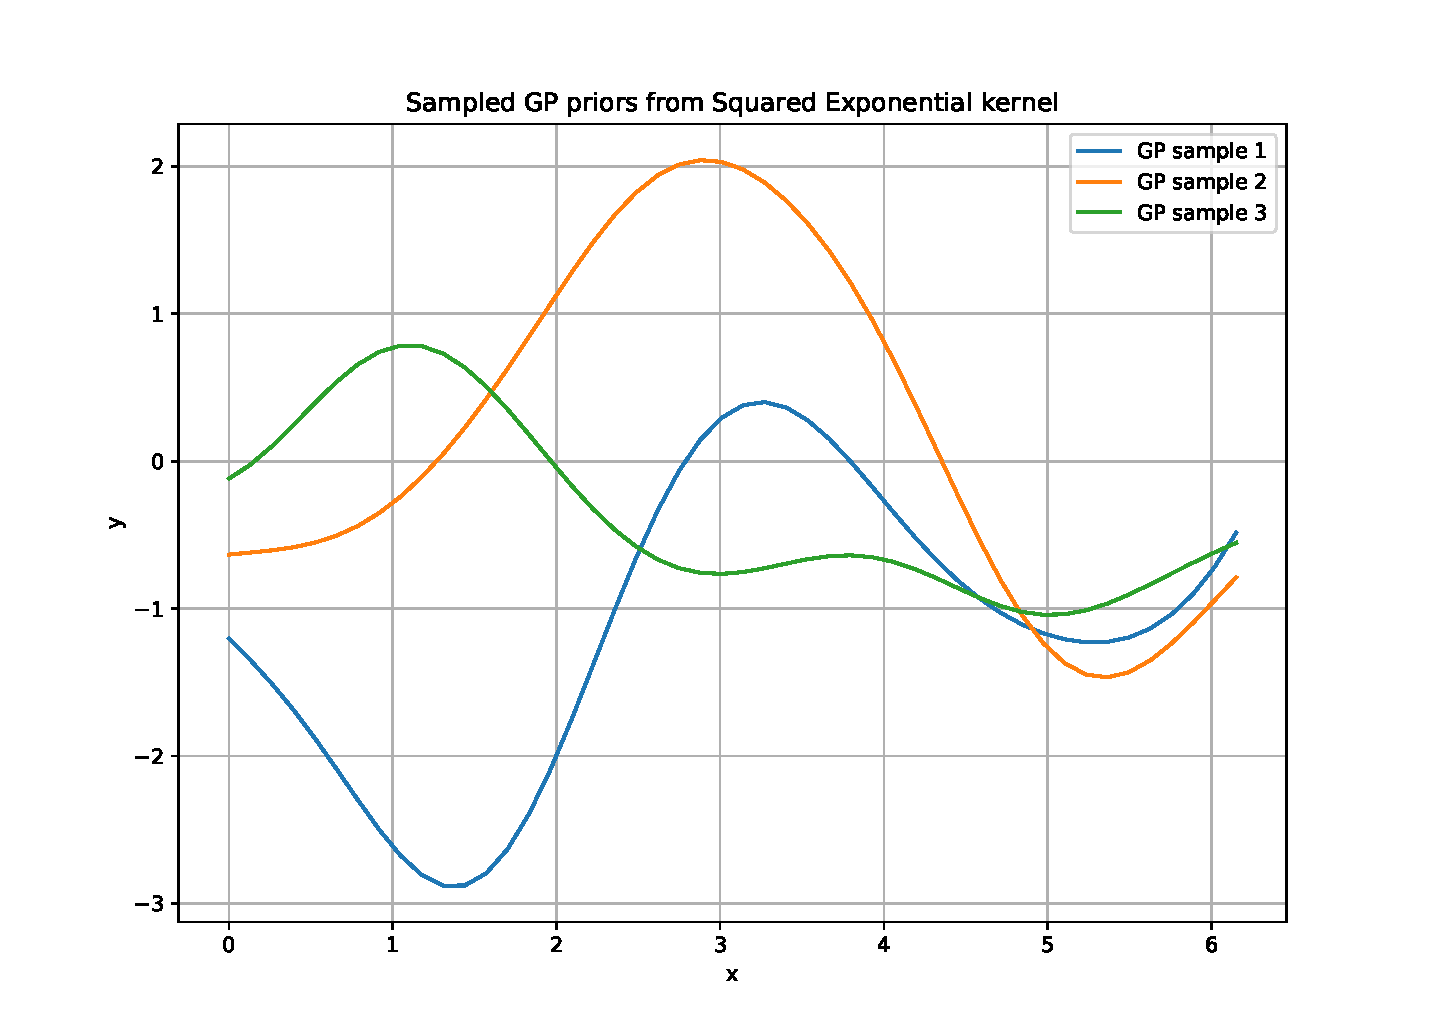
\includegraphics[width=\textwidth]{figures/chapter2/drawPrior}
\end{figure}

There's one important concept to explain before we move on. Notice in Figure \ref{fig:drawPrior} that the drawn functions seem to have a characteristic length-scale. This can be interpreted as the distance you have to move in input space before the function value changes significantly. By default, the squared exponential kernel uses a characteristic length-scale of 1 ($l = 1$). To change this behaviour to another, it is sufficient to consider $r/l$ instead of $r$ in Equation \ref{sqexp}. This can be thought as an hyperparameter to optimize, but we will return to this in another section.

\section{Prediction using a Gaussian Process prior}
\label{pred}

This is probably the most important section in this chapter. We will learn how to incorporate the knowledge of training data $D = \left\lbrace \left(\boldsymbol{x_i}, y_i\right) | i = 1,\dots,n\right\rbrace$ into our Gaussian Process to obtain a posterior predictive distribution. We will start considering the case that we have a noiseless function, that is to say, when $\sigma^2_n = 0$. Let us define $K(X, X_{*})$, the covariance function evaluated on train and test points, $K(X, X)$ the covariance function evaluated at only the training points, $K(X_{*}, X_{*})$ equivalently defined for the test values. Notice the last two have to be square matrices by definition.\\

Let us also use the following theorem:

\begin{mydef}
\label{conditioning}
Let $\boldsymbol{x}$ and $\boldsymbol{y}$ be jointly Gaussian:
\begin{equation}
\begin{bmatrix}
\boldsymbol{x}\\
\boldsymbol{y}
\end{bmatrix} \sim N\left(
\begin{bmatrix}
\boldsymbol{\mu_x}\\
\boldsymbol{\mu_y}
\end{bmatrix},
\begin{bmatrix}
A   && C \\
C^T && B
\end{bmatrix}
\right)
\end{equation}

Then $\boldsymbol{x|y} \sim \left(\boldsymbol{\mu_x} + C B^{-1}(\boldsymbol{y} - \boldsymbol{\mu_y}), A - CB^{-1}C^T \right)$
\end{mydef}

The reader might already be guessing what we are about to do now in terms of the training output points $\boldsymbol{f}$ and the corresponding testing points $\boldsymbol{f_*}$. According to the prior chosen in \ref{fprior}, assume that $\boldsymbol{f}$ and $\boldsymbol{f_*}$ are jointly Gaussian:

\begin{equation}
\begin{bmatrix}
\boldsymbol{f}\\
\boldsymbol{f_*}
\end{bmatrix} \sim N\left(
\boldsymbol{0},
\begin{bmatrix}
K(X, X)  && K(X, X_*) \\
K(X_*, X) && K(X_*, X_*)
\end{bmatrix}
\right)
\end{equation}


We are interested now in the distribution of $\boldsymbol{f_{*}}|\boldsymbol{f}$. Simply applying Theorem \ref{conditioning}, we can obtain:

\begin{equation}
\boldsymbol{f_*|f} \sim N\left(K(X_*, X)K(X, X)^{-1}\boldsymbol{f}, K(X_*, X_*) - K(X_*, X)K(X, X)^{-1}K(X, X_*) \right)
\end{equation}

This is pretty much everything basic there is to know about Gaussian Process estimation for regression. Now we have a complete predictive distribution over test values $\boldsymbol{f_{*}}$, and we can do with it what we please. For example, one could obtain an estimate of this function by drawing samples from a multivariate normal with the computed posterior parameters, or obtain a MAP estimate using the posterior mean.\\

Let us now consider the scenario where observations are not noise-free, that is, each time you query the function there is a i.i.d Gaussian error with mean $0$ and variance $\sigma_n^2 > 0$. Assume now the following prior on the noisy observations:

\begin{equation}
Cov(\boldsymbol{y}) = K(X, X) + \sigma^2_n I 
\end{equation}

Following the exact same math as before, but taking into account this new term, we got the following joint distribution:

\begin{equation}
\begin{bmatrix}
\boldsymbol{f}\\
\boldsymbol{f_*}
\end{bmatrix} \sim N\left(
\boldsymbol{0},
\begin{bmatrix}
K(X, X) + \sigma^2_n I && K(X, X_*) \\
K(X_*, X) && K(X_*, X_*)
\end{bmatrix}
\right)
\end{equation}

And conditioning again $\boldsymbol{f_{*}}$ on $\boldsymbol{f}$, we obtain our final predictive distribution:

\begin{equation}
\boldsymbol{f_*|f} \sim N(\boldsymbol{\overline{f_*}},  Cov(\boldsymbol{f_*}))
\end{equation}

where now:

\begin{align}
\boldsymbol{\overline{f_*}} = K(X_*, X)\left(K(X, X) + \sigma^2_n I   \right)^{-1}\boldsymbol{y}\\
Cov(\boldsymbol{f_*}) = K(X_*, X_*) - K(X_*, X)\left(K(X, X) + \sigma_n^2 I \right)^{-1}K(X, X_*)
\end{align}

It will probably be useful to note that a Gaussian Process model can be written easily in terms of a Bayesian hierarchical model, since:

\begin{align}
\label{hierarchical}
\boldsymbol{y}|\boldsymbol{f} \sim N(\boldsymbol{f}, \sigma^2_n I)\\
\label{hierarchical2}
\boldsymbol{f}|X \sim N(\boldsymbol{0}, K(X, X))
\end{align}

In fact, one can also assume other priors, even over $\sigma_n^2$. This representation may help us understand the introduction of the \textit{marginal likelihood}. This marginal likelihood in a Gaussian Process setting is defined as:

\begin{equation}
p(\boldsymbol{y}|X) = \int p(\boldsymbol{y}|\boldsymbol{f}, X)p(\boldsymbol{f}|X) d\boldsymbol{f}
\end{equation}

Using the results from Equations \ref{hierarchical} and \ref{hierarchical2} we can derive the integral analytically to obtain:

\begin{equation}
\log p(\boldsymbol{y}|X) = - \dfrac{1}{2}\boldsymbol{y}^T(K + \sigma^2_n I)^{-1}\boldsymbol{y} - \dfrac{1}{2}\log |K + \sigma^2_n I| - \dfrac{n}{2}\log 2\pi
\end{equation}

We have now all the necessary ingredients to lay down pseudo-code for your own implementation of a Gaussian Process regressor, as presented in Algorithm \ref{alg}. It makes use of several tricks for computational stability, such as a Cholesky decomposition and several linear system of equations to avoid directly inverting matrices.\\

\begin{algorithm}
	\caption{Gaussian regressor pseudo-code.}
		\label{alg}
		\begin{algorithmic}[1]
			\Function {GPRegressor}{$X$, $\boldsymbol{y}$, $k$, $\sigma_n^2$, $\boldsymbol{x_*}$}
			\State{$L \gets \textrm{chol}(K + \sigma_n^2 I)$}
			\State{$\boldsymbol{\alpha} \gets \textrm{linsolve}\left(L^T, \textrm{linsolve}(L, \boldsymbol{y})\right)$}
			\State{$\overline{f_*} \gets \boldsymbol{k_*}^T\boldsymbol{\alpha}$}
			\State{$\boldsymbol{v} \gets \textrm{linsolve}(L, \boldsymbol{k_*})$}
			\State{$\mathbb{V}\left[f_* \right] \gets k(\boldsymbol{x_*}, \boldsymbol{x_*}) - \boldsymbol{v}^T\boldsymbol{v}$}
			\State{$\log p(\boldsymbol{y}|X) \gets -\dfrac{1}{2}\boldsymbol{y}^T\boldsymbol{\alpha} - \sum_i \log L_{ii} - \dfrac{n}{2}\log 2\pi$}
			\EndFunction
		\end{algorithmic}
\end{algorithm}

pyGPGO includes an implementation of a Gaussian Process regressor under the \texttt{GPRegressor} module. A minimal working skeleton of its code is shown below. We do now show the entirety of the module code since most of it is not relevant at this point.

\begin{minted}[mathescape,
               linenos,
               numbersep=5pt,
               gobble=0,
               frame=lines,
               framesep=2mm,
               python3 = true]{python}
               
import numpy as np
from scipy.linalg import cholesky, solve
from collections import OrderedDict
from scipy.optimize import minimize

class GPRegressor:
        def __init__(self, covfunc, sigma = 0):
                self.covfunc = covfunc
                self.sigma = sigma
        def fit(self, X, y):
                self.X = X
                self.y = y
                self.nsamples = self.X.shape[0]
                self.K = self.covfunc.K(self.X, self.X)
                self.L = cholesky(self.K + self.sigma * np.eye(self.nsamples)).T
                self.alpha = solve(self.L.T, solve(self.L, y))
                self.logp = -.5 * np.dot(self.y, self.alpha) - np.sum(np.log(np.diag(self.L)))
                 - self.nsamples/2 * np.log(2 * np.pi)

        def predict(self, Xstar, return_std = False):
                Xstar = np.atleast_2d(Xstar)
                kstar = self.covfunc.K(self.X, Xstar).T
                fmean = np.dot(kstar, self.alpha)
                v = solve(self.L, kstar.T)
                fcov = self.covfunc.K(Xstar, Xstar) - np.dot(v.T, v)
                if return_std:
                        fcov = np.diag(fcov)
                return fmean, fcov

        def update(self, xnew, ynew):
                y = np.concatenate((self.y, ynew), axis = 0)
                X = np.concatenate((self.X, xnew), axis = 0)
                self.fit(X, y)
\end{minted}

A few notes on the code, first notice that the \texttt{GPRegressor} class only takes as input the covariance function to use $k$, and the noise level $\sigma_n^2$. It is only when you call the \texttt{fit} method on the function when you actually fit the model on some data $X, \boldsymbol{y}$. Quantities like the log-marginal likelihood are store within the object. The \texttt{predict} method not only can output the variance for a single prediction, but the covariance matrix for $m$ new ones if asked to. For convenience, we also implement an \texttt{update} method to update the Gaussian Process parameters when new data is available to us.

\subsection{A toy example of Gaussian Process regression}

Now that we have both the algorithm and the tools at hand, it may be interesting how a Gaussian Process regressor behaves with a toy example. We try to approximate a simple sine function in the interval $[0, 2\pi]$, and plot both the posterior mean and a 95\% confidence band using the posterior variance of the fitted process. The code shown below produces Figure \ref{fig:GPsine}.

\newpage

\begin{minted}[mathescape,
               linenos,
               numbersep=5pt,
               gobble=0,
               frame=lines,
               framesep=2mm,
               python3 = true]{python}

import numpy as np
from GPRegressor import GPRegressor
from covfunc import squaredExponential
import matplotlib.pyplot as plt


if __name__ == '__main__':
        # Build synthetic data (sine function)
        x = np.arange(0, 2 * np.pi + 0.01, step = np.pi / 2)
        y = np.sin(x)
        X = np.array([np.atleast_2d(u) for u in x])[:, 0]

        # Specify covariance function
        sexp = squaredExponential()
        # Instantiate GPRegressor class
        gp = GPRegressor(sexp)
        # Fit the model to the data
        gp.fit(X, y)

        # Predict on new data
        xstar = np.arange(0, 2*np.pi, step = 0.01)
        Xstar = np.array([np.atleast_2d(u) for u in xstar])[:, 0]
        ymean, ystd = gp.predict(Xstar, return_std = True)

        # Confidence interval bounds
        lower, upper = ymean - 1.96 * ystd, ymean + 1.96 * ystd

        # Plot values
        plt.figure()
        plt.plot(xstar, ymean, label = 'Posterior mean')
        plt.plot(xstar, np.sin(xstar), label = 'True function')
        plt.fill_between(xstar, lower, upper, alpha = 0.4, label = '95% confidence band')
        plt.grid()
        plt.legend(loc = 0)
        plt.show()
\end{minted}

\begin{figure}
\caption{A fitted Gaussian Process regressor to samples of the sine function.}
\label{fig:GPsine}
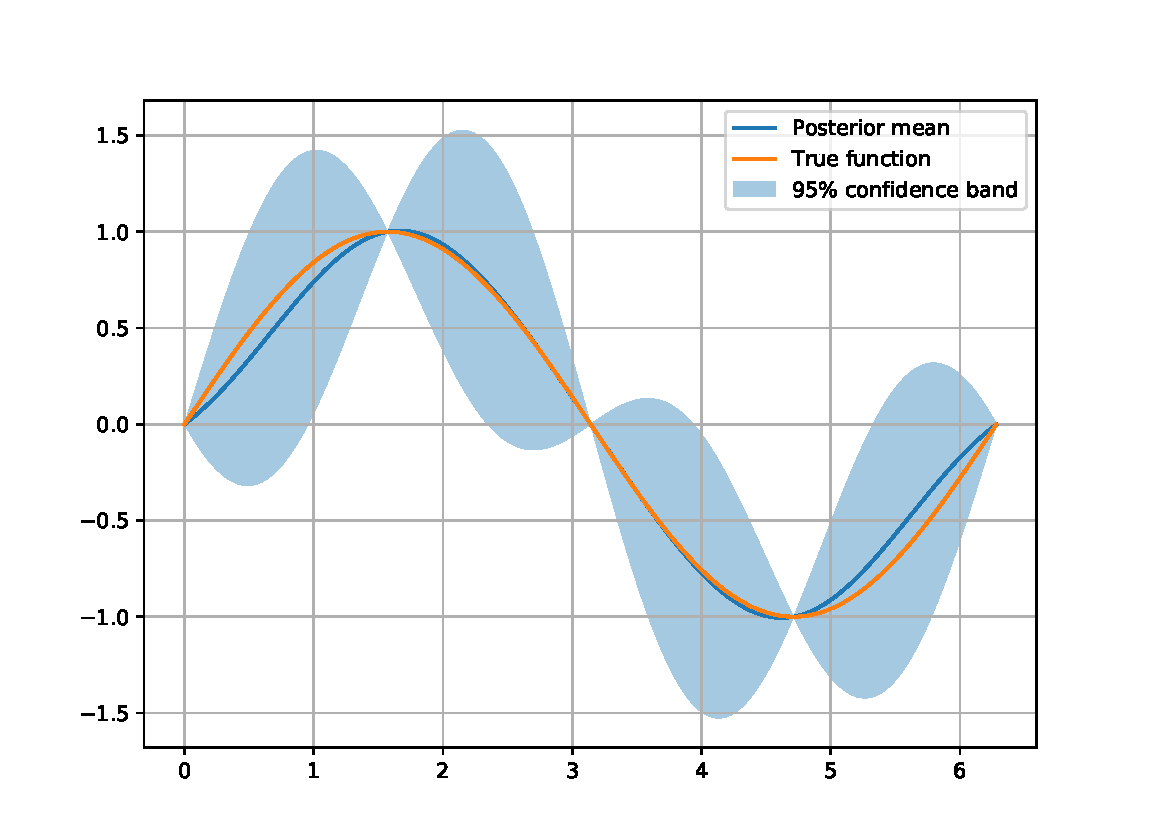
\includegraphics[width=\textwidth]{figures/chapter2/GPsine}
\end{figure}

\section{On covariance functions}

A covariance function, like the squared exponential kernel that we have been using as a example throughout the chapter encodes our assumptions of similarity between inputs from $\boldsymbol{x}$. We assume \textit{similar} items in input space to have similar values of the target value $y$. Not any function of $\boldsymbol{x}$ and $\boldsymbol{x'}$ can be considered a covariance function, in general should fulfil properties like the following:

\begin{itemize}
\item \textit{Stationarity}. A covariance function is said to be stationary if it is a function of $|\boldsymbol{x} - \boldsymbol{x'}|$. That is to say that it is invariant to translations in the input space. Most of the covariance functions we will see fall into this category.
\item \textit{Isotropy}. A covariance function is said to be isotropic if it is \textit{only} function of  $|\boldsymbol{x} - \boldsymbol{x'}|$. Therefore, every isotropic covariance function is stationary.
\item Dot-product. Some covariance functions are functionals of the dot-product $|\boldsymbol{x}^T \boldsymbol{x'}|$. These kernels, while invariant to rotations are not invariant to translations.
\end{itemize}

There is an excellent theoretical analysis of covariance functions in Chapter 4 of Carl E. Rasmussen's book \textit{Gaussian Processes for Machine Learning}. We will not cover this here since it falls beyond the scope of this manual. However, we will start providing examples of the most common covariance functions and their implementation in pyGPGO.\\

The \textit{Squared Exponential} covariance function is the one that we have been using so far. It is also arguably the most used in practice. It takes the general form:

\begin{equation}
k_{SE}(r) = \exp\left(-\dfrac{r^2}{2l^2} \right)
\end{equation}

Where $l$ is the parameter controlling its characteristic length-scale. It is useful to define these functions in terms of $r$ since we can abstract this calculation to another function. A simple skeleton of its implementation in pyGPGO is the following:

\begin{minted}[mathescape,
               linenos,
               numbersep=5pt,
               gobble=0,
               frame=lines,
               framesep=2mm,
               python3 = true]{python}
import numpy as np
from scipy.special import gamma, kv
from scipy.spatial.distance import cdist

def l2norm_(X, Xstar):
        return cdist(X, Xstar)

class squaredExponential:
        def __init__(self, l = 1, sigma2f = 1, sigma2n = 0):
                self.l = l
                self.sigma2f = sigma2f
                self.sigma2n = sigma2n

        def K(self, X, Xstar):
                r = l2norm_(X, Xstar)
                return(np.exp(-.5 * r ** 2 / self.l ** 2))
\end{minted}

The \textit{Matern class} of covariance functions takes the form:

\begin{equation}
k_{\textrm{Matern}}(r) = \dfrac{2^{1-\nu}}{\Gamma(\nu)}\left(\dfrac{\sqrt{2\nu} r}{l}    \right)^\nu K_\nu\left( \dfrac{\sqrt{2\nu}r}{l} \right)
\end{equation}

with $\nu, l > 0$ and $K_\nu$ is a modified Bessel function of the second kind. Notice that if we take limit $\nu \rightarrow \infty$ we obtain our beloved squared exponential covariance function. pyGPGO implementation below.

\begin{minted}[mathescape,
               linenos,
               numbersep=5pt,
               gobble=0,
               frame=lines,
               framesep=2mm,
               python3 = true]{python}
class matern:
        def __init__(self, v = 1, l = 1):
                self.v, self.l = v, l

        def K(self, X, Xstar):
                r = l2norm_(x, xstar)
                bessel = kv(self.v, np.sqrt(2 * self.v) * r / self.f)
                f = 2 ** (1 - self.v) / gamma(self.v) * 
                	(np.sqrt(2 * self.v) * r / self.l) ** self.v
                res = f * bessel
                res[np.isnan(res)] = 1
                return(res)               
\end{minted}

The $\gamma$-exponential covariance function, of which the squared exponential is a special case. It takes the general form:

\begin{equation}
k(r) = \exp\left( - \left(\dfrac{r}{l}\right)^\gamma  \right)
\end{equation}

for $0 < \gamma \leq 2$. Its implementation in pyGPGO below:

\begin{minted}[mathescape,
               linenos,
               numbersep=5pt,
               gobble=0,
               frame=lines,
               framesep=2mm,
               python3 = true]{python}               
class gammaExponential:
        def __init__(self, gamma = 1, l = 1):
                self.gamma = gamma
                self.l = l

        def K(self, X, Xstar):
                r = l2norm_(X, Xstar)
                return(np.exp(-(r / self.l) ** self.gamma))              
\end{minted}

The \textit{Rational Quadratic} covariance function takes the form:

\begin{equation}
k_{RQ}(r) = \left( 1 + \dfrac{r^2}{2\alpha l^2} \right)^{-\alpha}
\end{equation}

with $\alpha, l > 0$. And again its implementation:

\begin{minted}[mathescape,
               linenos,
               numbersep=5pt,
               gobble=0,
               frame=lines,
               framesep=2mm,
               python3 = true]{python}
class rationalQuadratic:
        def __init__(self, alpha = 1, l = 1):
                self.alpha = alpha
                self.l = l

        def K(self, X, Xstar):
                r = l2norm_(X, Xstar)
                return((1 + r**2/(2 * self.alpha * self.l **2))**(-self.alpha))  
\end{minted}

The \textit{arcSin} kernel is an example of a dot product covariance function, therefore non-stationary:

\begin{equation}
k_{\textrm{arcSin}}(\boldsymbol{x}, \boldsymbol{x'}) = \dfrac{2}{\pi}\sin^{-1}\left(\dfrac{2\boldsymbol{x}\Sigma\boldsymbol{x'}}{\sqrt{(1 + 2\boldsymbol{x}^T\Sigma\boldsymbol{x})(1 + 2\boldsymbol{x'}^T\Sigma\boldsymbol{x})}}   \right)
\end{equation}

And I promise this is the final covariance function implementation in this section.

\begin{minted}[mathescape,
               linenos,
               numbersep=5pt,
               gobble=0,
               frame=lines,
               framesep=2mm,
               python3 = true]{python}
class arcSin:
        def __init__(self, n, sigma = None):
                if sigma == None:
                        self.sigma = np.eye(n)
                else:
                        self.sigma = sigma
        def k(self, x, xstar):
                num = 2 * np.dot(np.dot(x[np.newaxis, :], self.sigma), xstar)
                a = 1 + 2 * np.dot(np.dot(x[np.newaxis, :], self.sigma), x)
                b = 1 + 2 * np.dot(np.dot(xstar[np.newaxis, :], self.sigma), xstar)
                res = num / np.sqrt(a * b)
                return(res)
   
\end{minted}

\subsection{A zoo of covariance functions}

We have seen plenty of covariance function specifications in the last section. Remember that these control the degree of \textit{similarity} between input points. As an exercise, it would be good to recreate the same sine function example that we saw before, using four different stationary different covariance functions. The choice of parameters is the default one in pyGPGO. The script shown below produces Figure \ref{fig:zoo}. 

\begin{minted}[mathescape,
               linenos,
               numbersep=5pt,
               gobble=0,
               frame=lines,
               framesep=2mm,
               python3 = true]{python}
import numpy as np
from covfunc import *
from GPRegressor import GPRegressor
import matplotlib.pyplot as plt


if __name__ == '__main__':
        # Build synthetic data (sine function)
        x = np.arange(0, 2 * np.pi + 0.01, step = np.pi / 2)
        y = np.sin(x)
        X = np.array([np.atleast_2d(u) for u in x])[:, 0]

        # Covariance functions to loop over
        covfuncs = [squaredExponential(), matern(), gammaExponential(), rationalQuadratic()]
        titles = [r'Squared Exponential ($l = 1$)', r'Matern ($\nu = 1$, $l = 1$)',
         r'Gamma Exponential ($\gamma = 1, l = 1$)', r'Rational Quadratic ($\alpha = 1, l = 1$)']
        plt.figure()
        plt.rc('text', usetex=True)
        for i, cov in enumerate(covfuncs):
                gp = GPRegressor(cov)
                gp.fit(X, y)
                xstar = np.arange(0, 2 * np.pi, step = 0.01)
                Xstar = np.array([np.atleast_2d(u) for u in xstar])[:, 0]
                ymean, ystd = gp.predict(Xstar, return_std = True)
                
                lower, upper = ymean - 1.96 * ystd, ymean + 1.96 * ystd
                plt.subplot(2, 2, i + 1)
                plt.plot(xstar, ymean, label = 'Posterior mean')
                plt.plot(xstar, np.sin(xstar), label = 'True function')
                plt.fill_between(xstar, lower, upper, alpha = 0.4,
                 label = '95\% confidence band')
                plt.grid()
                plt.title(titles[i])
        plt.legend(loc = 0)
        plt.show()
\end{minted}

\begin{figure}
\caption{Behaviour of different stationary covariance functions with the default parameters in pyGPGO.}
\label{fig:zoo}
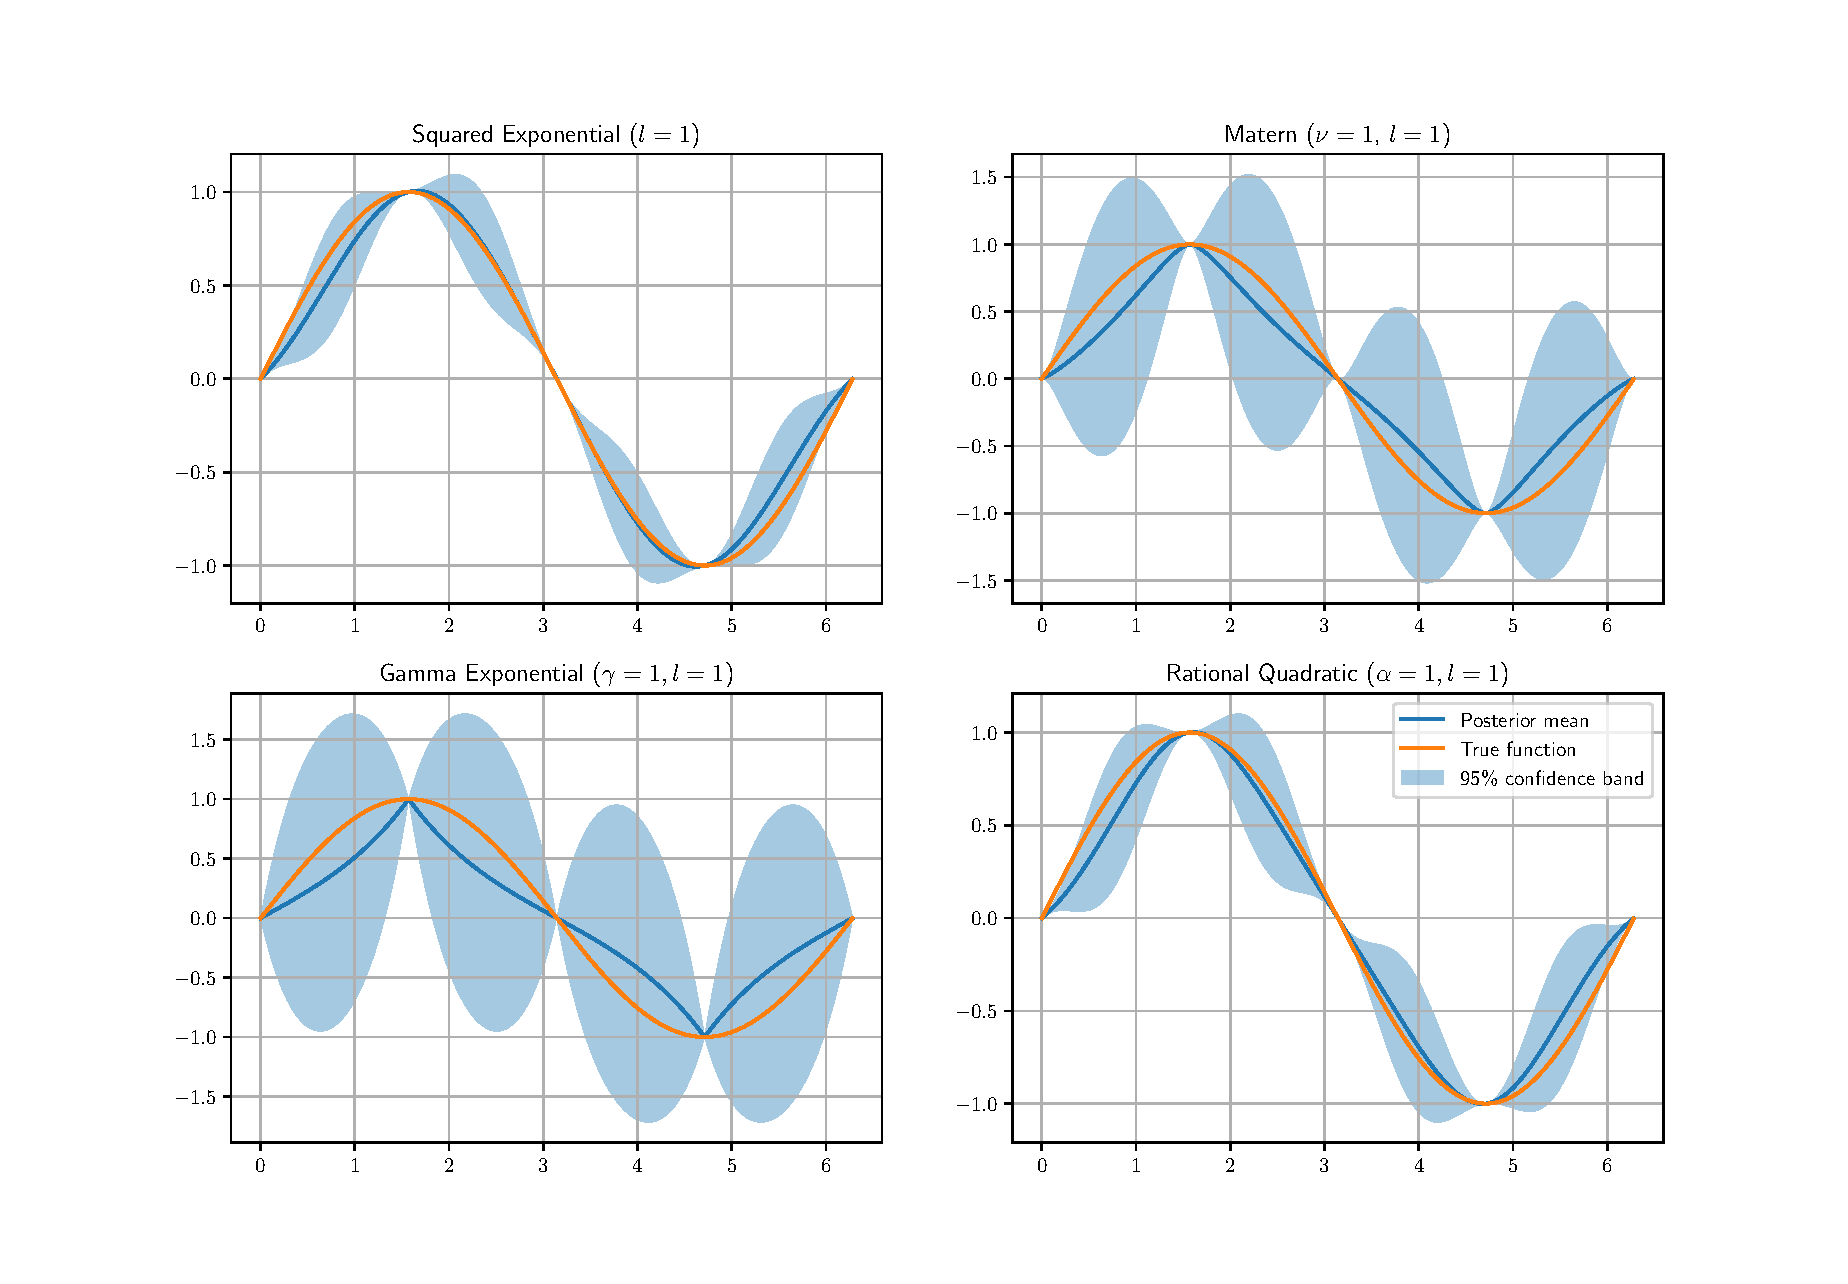
\includegraphics[width=\textwidth]{figures/chapter2/zoo}
\end{figure}

\section{Hyperparameter optimization}

As seen in the previous sections, different covariance functions have different \textit{hyperparameters}. These control how the kernel measures similarity among different instances of $\boldsymbol{x}$. So far, we have chosen these hyperparameters according to those set default in pyGPGO, but one may want to optimize these according to the data they have at hand. Depending on the situation, this optimization may lead to better models, either in terms of accuracy or interpretability. There are several ways to select these hyperparameters, one more analytical, by optimizing the marginal log-likelihood, and simpler ones based on cross-validation.

\subsection{Type II Maximum Likelihood}

This is the Bayesian analytical approach to optimizing hyperparameters. One may quickly notice that Gaussian Processes are non-parametric models, in the sense that apart from the quantities set in the covariance functions, there is nothing else to optimize for. First we will provide a small background on Bayesian model selection. Assume that we have a model  $\mathcal{H}_i$ with \textit{parameters} $\boldsymbol{w}$, \textit{hyperparameters} $\boldsymbol{\theta}$, and we have some training data $X, \boldsymbol{y}$. The posterior over the parameters is easily given by:

\begin{equation}
\label{posteriorparam}
p(\boldsymbol{w}|\boldsymbol{y}, X, \boldsymbol{\theta}, \mathcal{H}_i) = \dfrac{p(\boldsymbol{y}|X, \boldsymbol{w}, \mathcal{H}_i)p(\boldsymbol{w}|\boldsymbol{\theta}, \mathcal{H}_i)}{p(\boldsymbol{y}|X, \boldsymbol{\theta}, \mathcal{H}_i)}
\end{equation}

where $p(\boldsymbol{y}|X, \boldsymbol{w}, \mathcal{H}_i)$ is the likelihood, $p(\boldsymbol{w}|\boldsymbol{\theta}, \mathcal{H}_i)$ our prior distribution over the parameters and $p(\boldsymbol{y}|X, \boldsymbol{\theta}, \mathcal{H}_i)$ is called the \textit{evidence} or marginal likelihood. Notice that this last quantity is nothing but the integral over parameter space of the numerator in Equation \ref{posteriorparam}.\\

We can do the same at the next level of inference for the hyperparameters. The posterior of hyperparameters is defined as:

\begin{equation}
\label{posteriorhyper}
p(\boldsymbol{\theta}|\boldsymbol{y}, X, \mathcal{H}_i) = \dfrac{p(\boldsymbol{y}|X, \boldsymbol{\theta}, \mathcal{H}_i)p(\boldsymbol{\theta}|\mathcal{H}_i)}{p(\boldsymbol{y}|X, \mathcal{H}_i)}
\end{equation}

where now $p(\boldsymbol{\theta}|\mathcal{H}_i)$ is our prior over hyperparameters. We are interested however in optimizing the denominator in Equation \ref{posteriorhyper} with respect to the hyperparameters. Typically, in Bayesian inference to perform the kind of integrals presented before, one has to resort to sampling procedures related to Markov Chain Monte Carlo, such as the Gibbs sampler. In the case of Gaussian processes, all computations are analytically tractable. In fact, the expression of the marginal likelihood was presented in Section \ref{pred}. We reproduce the expression here for completeness:

\begin{equation}
\log p(\boldsymbol{y}|X) = - \dfrac{1}{2}\boldsymbol{y}^T(K + \sigma^2_n I)^{-1}\boldsymbol{y} - \dfrac{1}{2}\log |K + \sigma^2_n I| - \dfrac{n}{2}\log 2\pi
\end{equation}

For typical local optimization methods to work fairly well, we may also need an specification of the derivative of the log-marginal likelihood w.r.t. the hyperparameters.

\begin{equation}
\dfrac{\partial}{\partial \theta_j}\log p(\boldsymbol{y}|X, \boldsymbol{\theta}) = \dfrac{1}{2}\boldsymbol{y}^T K^{-1}\dfrac{\partial K}{\partial \theta_j}K^{-1}\boldsymbol{y} - \dfrac{1}{2}\textrm{tr}\left(K^{-1} \dfrac{\partial K}{\partial \theta_j} \right)
\end{equation}

where $\dfrac{\partial K}{\partial \theta_j}$ denotes the derivative of the selected covariance function, evaluated at each pair of instances of the training set. For optimization, one may choose to make use of this expression or not, depending on both of the optimization algorithm (gradient ascent, L-BFGS-B...) or on the cost of evaluation of the derivative. In pyGPGO, most of the covariance functions are implemented with a method \texttt{gradK} to return the gradient, for example, the complete specification of the \texttt{squaredExponential} class is:

\begin{minted}[mathescape,
               linenos,
               numbersep=5pt,
               gobble=0,
               frame=lines,
               framesep=2mm,
               python3 = true]{python}
class squaredExponential:
        def __init__(self, l = 1, sigma2f = 1, sigma2n = 0):
                self.l = l
                self.sigma2f = sigma2f
                self.sigma2n = sigma2n

        def K(self, X, Xstar):
                r = l2norm_(X, Xstar)
                return(np.exp(-.5 * r ** 2 / self.l ** 2))

        def gradK(self, X, Xstar, param = 'l'):
                if param == 'l':
                        r = l2norm_(X, Xstar)
                        num = r**2 * np.exp(-r**2 /(2* self.l**2))
                        den = self.l ** 3
                        l_grad = num / den
                        return(l_grad)
                else:
                        raise ValueError('Param not found')               
\end{minted}

By default, the \texttt{GPRegressor} class in pyGPGO does no hyperparameter optimization unless explicitly asked to. If the gradient of the covariance function is available, it will make use of it, if not, it will be estimated in a numerical fashion using the L-BFGS-B algorithm.


\subsubsection{Another toy example: Optimizing the characteristic length-scale}

To illustrate the previous point, it may be a good idea to see the behaviour of the marginal log-likelihood and its gradient when we modify the characteristic length scale $l$ in the squared exponential covariance function. The sine function will also serve as playground here. The code below produces Figure \ref{fig:logmarginal}.

\begin{minted}[mathescape,
               linenos,
               numbersep=5pt,
               gobble=0,
               frame=lines,
               framesep=2mm,
               python3 = true]{python}
import numpy as np
from GPRegressor import GPRegressor
from covfunc import squaredExponential
import matplotlib.pyplot as plt

def gradient(gp, sexp):
        alpha = gp.alpha
        K = gp.K
        gradK = sexp.gradK(gp.X, gp.X, 'l')
        inner = np.dot(np.atleast_2d(alpha).T, np.atleast_2d(alpha)) - np.linalg.inv(K)
        return(.5 * np.trace(np.dot(inner, gradK)))


if __name__ == '__main__':
        x = np.arange(0, 2 * np.pi + 0.01, step = np.pi / 2)
        X = np.array([np.atleast_2d(u) for u in x])[:, 0]
        y = np.sin(x)

        logp = []
        grad = []
        length_scales = np.linspace(0.1, 2, 1000)

        for l in length_scales:
                sexp = squaredExponential(l = l)
                gp = GPRegressor(sexp)
                gp.fit(X, y)
                logp.append(gp.logp)
                grad.append(gradient(gp, sexp))

        plt.figure()
        plt.subplot(2, 1, 1)
        plt.plot(length_scales, logp)
        plt.title('Marginal log-likelihood')
        plt.xlabel('Characteristic length-scale l')
        plt.ylabel('log-likelihood')
        plt.grid()
        plt.subplot(2, 1, 2)
        plt.plot(length_scales, grad, '--', color = 'red')
        plt.title('Gradient w.r.t. l')
        plt.xlabel('Characteristic length-scale l')
        plt.grid()
        plt.show()
\end{minted}
\FloatBarrier

\begin{figure}
\caption{Log-marginal likelihood and its gradient w.r.t to the characteristic length-scale. Notice there seems to be an optimal point at around $l = 1.4$.}
\label{fig:logmarginal}
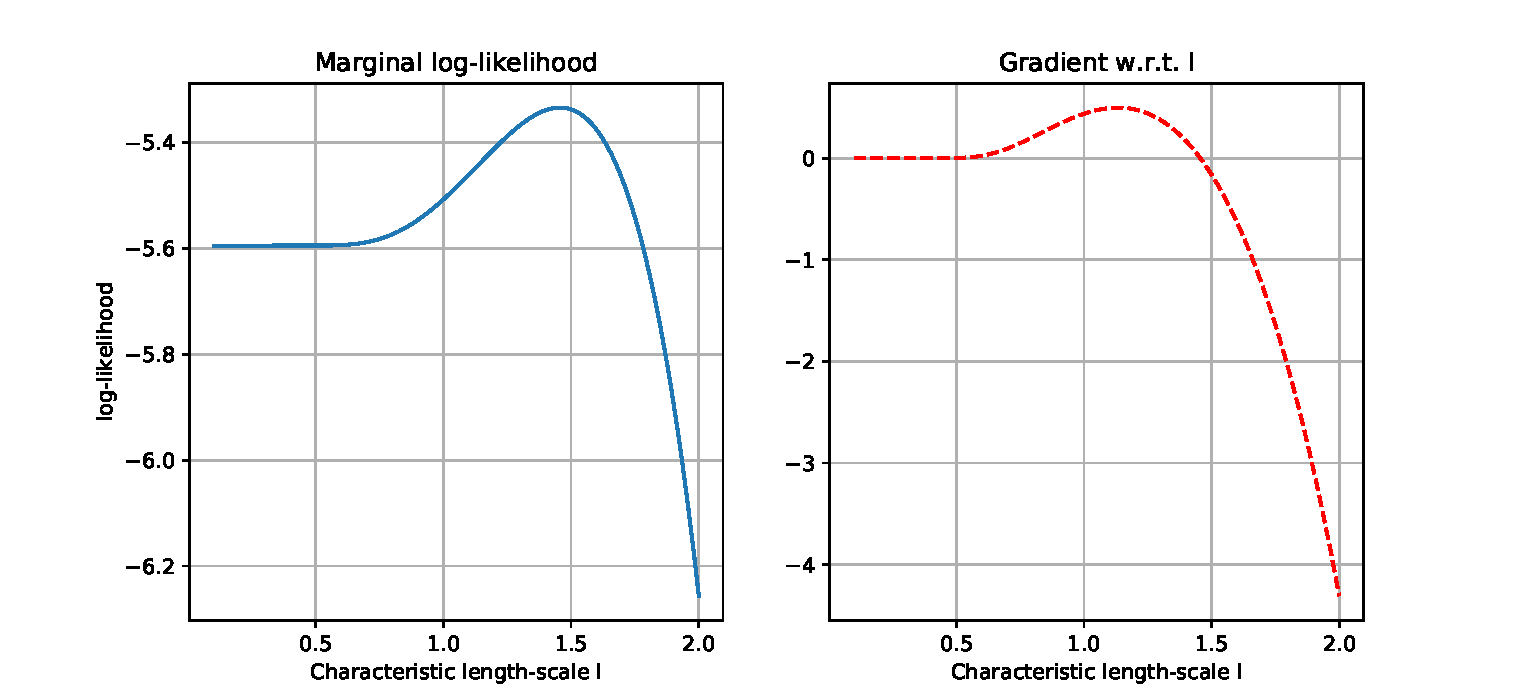
\includegraphics[width=\textwidth]{figures/chapter2/logmarginal}
\end{figure}

\subsection{Cross validation}

There is a very extensive analytical evaluation of cross validation using Gaussian Process in Rasmussen's book. Here, we will only lay down some very basic ideas related to model selection from a very basic machine learning perspective. The concepts presented here should not be new to the reader, but are more useful if one plans to use Gaussian Processes only as a regression model, not as a surrogate one towards another objective, as we will do in the following chapter. \\

To evaluate the performance of hyperparameters $\boldsymbol{\theta}$, in $D=\left( X, \boldsymbol{y}\right)$ one could do the following:

\begin{itemize}
\item \textbf{Holdout test}. Consider $D = \left\lbrace D_T, D_V \right\rbrace$ as a training and validation set from your data and $\boldsymbol{\nu}$ the set of hyperparameter vectors $\boldsymbol{\nu}$ to test. Train your Gaussian Process regressor on $D_T$ with some subset of hyperparameters from $\boldsymbol{\nu}$ and test its performance according to some loss metric $\mathcal{L}$ on $D_V$. Choose hyperparameters according to the lower loss obtained.
\item \textbf{$k$-fold cross validation}. Instead of considering a single test set $D_V$, partition $D={D_1,\dots, D_k}$. Train your model iteratively on $k-1$ sets and test on the remaining one. Consider an average of losses for each hyperparameter to test.  
\end{itemize}



\chapter{Bayesian optimization}
\chapter{Experiments}
\chapter{pyGPGO: A simple Python Package for Bayesian Optimization}

\end{document}